

\tikzset{every picture/.style={line width=0.75pt}} %set default line width to 0.75pt        

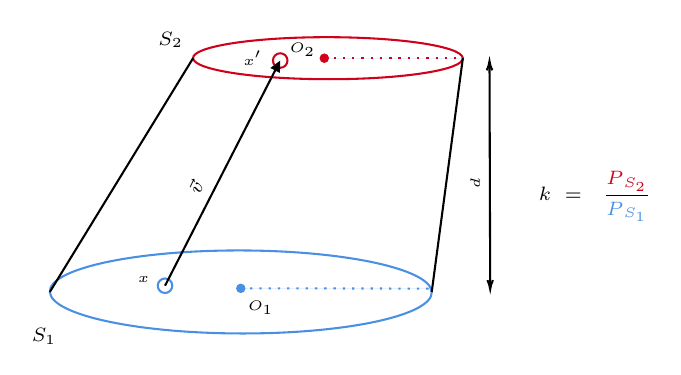
\begin{tikzpicture}[x=0.75pt,y=0.75pt,yscale=-1,xscale=1]
%uncomment if require: \path (0,300); %set diagram left start at 0, and has height of 300

%Shape: Ellipse [id:dp5388131408233692] 
\draw  [color={rgb, 255:red, 208; green, 2; blue, 27 }  ,draw opacity=1 ] (297.51,88.88) .. controls (297.23,83.28) and (326.1,78.75) .. (361.99,78.75) .. controls (397.89,78.75) and (427.21,83.28) .. (427.49,88.88) .. controls (427.77,94.47) and (398.9,99) .. (363.01,99) .. controls (327.11,99) and (297.79,94.47) .. (297.51,88.88) -- cycle ;
%Shape: Ellipse [id:dp777621474822027] 
\draw  [color={rgb, 255:red, 74; green, 144; blue, 226 }  ,draw opacity=1 ] (228.5,201.5) .. controls (227.95,190.45) and (268.69,181.5) .. (319.5,181.5) .. controls (370.31,181.5) and (411.95,190.45) .. (412.5,201.5) .. controls (413.05,212.55) and (372.31,221.5) .. (321.5,221.5) .. controls (270.69,221.5) and (229.05,212.55) .. (228.5,201.5) -- cycle ;
%Straight Lines [id:da6429244999105203] 
\draw    (297.51,88.88) -- (228.5,201.5) ;
%Straight Lines [id:da7997251507611736] 
\draw    (427.49,88.88) -- (412.5,201.5) ;
%Shape: Circle [id:dp47840542367844163] 
\draw  [color={rgb, 255:red, 208; green, 2; blue, 27 }  ,draw opacity=1 ] (336,90) .. controls (336,88.07) and (337.57,86.5) .. (339.5,86.5) .. controls (341.43,86.5) and (343,88.07) .. (343,90) .. controls (343,91.93) and (341.43,93.5) .. (339.5,93.5) .. controls (337.57,93.5) and (336,91.93) .. (336,90) -- cycle ;
%Shape: Circle [id:dp9835136469560248] 
\draw  [color={rgb, 255:red, 74; green, 144; blue, 226 }  ,draw opacity=1 ] (280.5,198.5) .. controls (280.5,196.57) and (282.07,195) .. (284,195) .. controls (285.93,195) and (287.5,196.57) .. (287.5,198.5) .. controls (287.5,200.43) and (285.93,202) .. (284,202) .. controls (282.07,202) and (280.5,200.43) .. (280.5,198.5) -- cycle ;
%Shape: Circle [id:dp283439076913375] 
\draw  [color={rgb, 255:red, 74; green, 144; blue, 226 }  ,draw opacity=1 ][fill={rgb, 255:red, 74; green, 144; blue, 226 }  ,fill opacity=1 ] (318.75,199.75) .. controls (318.75,198.78) and (319.53,198) .. (320.5,198) .. controls (321.47,198) and (322.25,198.78) .. (322.25,199.75) .. controls (322.25,200.72) and (321.47,201.5) .. (320.5,201.5) .. controls (319.53,201.5) and (318.75,200.72) .. (318.75,199.75) -- cycle ;
%Straight Lines [id:da48707589962772135] 
\draw [color={rgb, 255:red, 74; green, 144; blue, 226 }  ,draw opacity=1 ][fill={rgb, 255:red, 74; green, 144; blue, 226 }  ,fill opacity=1 ] [dash pattern={on 0.84pt off 2.51pt}]  (320.5,199.75) -- (412.5,199.88) ;
%Shape: Circle [id:dp49021214062686846] 
\draw  [color={rgb, 255:red, 208; green, 2; blue, 27 }  ,draw opacity=1 ][fill={rgb, 255:red, 208; green, 2; blue, 27 }  ,fill opacity=1 ] (359,88.88) .. controls (359,87.91) and (359.78,87.13) .. (360.75,87.13) .. controls (361.72,87.13) and (362.5,87.91) .. (362.5,88.88) .. controls (362.5,89.84) and (361.72,90.63) .. (360.75,90.63) .. controls (359.78,90.63) and (359,89.84) .. (359,88.88) -- cycle ;
%Straight Lines [id:da1367202995891349] 
\draw [color={rgb, 255:red, 208; green, 2; blue, 27 }  ,draw opacity=1 ][fill={rgb, 255:red, 74; green, 144; blue, 226 }  ,fill opacity=1 ] [dash pattern={on 0.84pt off 2.51pt}]  (360.75,88.88) -- (427.49,88.88) ;
%Straight Lines [id:da5349865593191481] 
\draw    (284,198.5) -- (338.13,92.67) ;
\draw [shift={(339.5,90)}, rotate = 117.09] [fill={rgb, 255:red, 0; green, 0; blue, 0 }  ][line width=0.08]  [draw opacity=0] (5.36,-2.57) -- (0,0) -- (5.36,2.57) -- cycle    ;
%Straight Lines [id:da26724130845467164] 
\draw [line width=0.75]    (440.34,92.33) -- (440.48,139.83) -- (440.5,144.17) -- (440.66,198.17) ;
\draw [shift={(440.67,200.17)}, rotate = 269.83] [color={rgb, 255:red, 0; green, 0; blue, 0 }  ][line width=0.75]    (4.37,-1.32) .. controls (2.78,-0.56) and (1.32,-0.12) .. (0,0) .. controls (1.32,0.12) and (2.78,0.56) .. (4.37,1.32)   ;
\draw [shift={(440.33,90.33)}, rotate = 89.83] [color={rgb, 255:red, 0; green, 0; blue, 0 }  ][line width=0.75]    (4.37,-1.32) .. controls (2.78,-0.56) and (1.32,-0.12) .. (0,0) .. controls (1.32,0.12) and (2.78,0.56) .. (4.37,1.32)   ;

% Text Node
\draw (218.33,217.67) node [anchor=north west][inner sep=0.75pt]  [font=\scriptsize] [align=left] {$\displaystyle S_{1}$};
% Text Node
\draw (279.33,74.67) node [anchor=north west][inner sep=0.75pt]  [font=\scriptsize] [align=left] {$\displaystyle S_{2}$};
% Text Node
\draw (269.53,192.73) node [anchor=north west][inner sep=0.75pt]  [font=\tiny] [align=left] {$\displaystyle x$};
% Text Node
\draw (320.33,84) node [anchor=north west][inner sep=0.75pt]  [font=\tiny] [align=left] {$\displaystyle x'$};
% Text Node
\draw (429.48,152.88) node [anchor=north west][inner sep=0.75pt]  [font=\tiny,rotate=-271.92] [align=left] {$\displaystyle d$};
% Text Node
\draw (462.67,142) node [anchor=north west][inner sep=0.75pt]  [font=\scriptsize] [align=left] {$\displaystyle k\ =\ \ \frac{\textcolor[rgb]{0.82,0.01,0.11}{P}\textcolor[rgb]{0.82,0.01,0.11}{_{S_{2}}}}{\textcolor[rgb]{0.29,0.56,0.89}{P}\textcolor[rgb]{0.29,0.56,0.89}{_{S_{1}}}}$};
% Text Node
\draw (292.58,152.91) node [anchor=north west][inner sep=0.75pt]  [font=\scriptsize,rotate=-296.11] [align=left] {$\displaystyle \vec{v}$};
% Text Node
\draw (322.5,204.5) node [anchor=north west][inner sep=0.75pt]  [font=\tiny] [align=left] {$\displaystyle O_{1}$};
% Text Node
\draw (342.69,80.01) node [anchor=north west][inner sep=0.75pt]  [font=\tiny] [align=left] {$\displaystyle O_{2}$};


\end{tikzpicture}
